% This file was created with tikzplotlib v0.10.1.
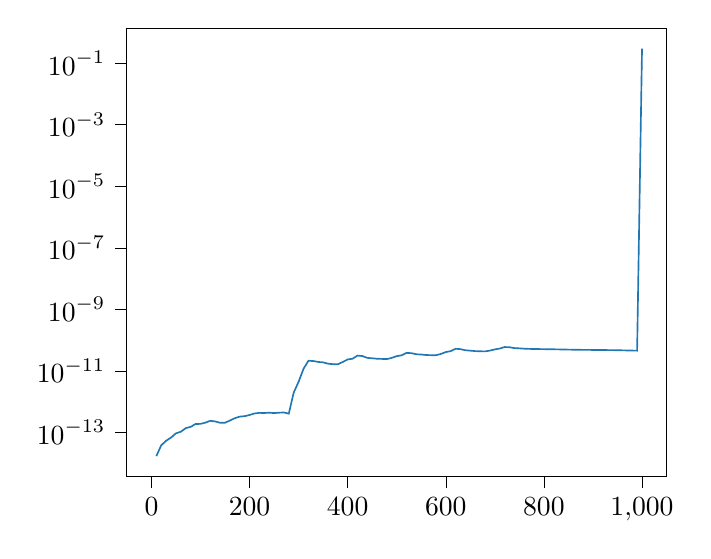
\begin{tikzpicture}

\definecolor{darkgray176}{RGB}{176,176,176}
\definecolor{steelblue31119180}{RGB}{31,119,180}

\begin{axis}[
log basis y={10},
tick align=outside,
tick pos=left,
x grid style={darkgray176},
xmin=-50, xmax=1050,
xtick style={color=black},
y grid style={darkgray176},
ymin=3.67340261954334e-15, ymax=1.36636556554865,
ymode=log,
ytick style={color=black},
ytick={1e-17,1e-15,1e-13,1e-11,1e-09,1e-07,1e-05,0.001,0.1,10,1000},
yticklabels={
  \(\displaystyle {10^{-17}}\),
  \(\displaystyle {10^{-15}}\),
  \(\displaystyle {10^{-13}}\),
  \(\displaystyle {10^{-11}}\),
  \(\displaystyle {10^{-9}}\),
  \(\displaystyle {10^{-7}}\),
  \(\displaystyle {10^{-5}}\),
  \(\displaystyle {10^{-3}}\),
  \(\displaystyle {10^{-1}}\),
  \(\displaystyle {10^{1}}\),
  \(\displaystyle {10^{3}}\)
}
]
\addplot [semithick, steelblue31119180]
table {%
10 1.68796684565683e-14
20 3.81311220678585e-14
30 5.35007440481041e-14
40 6.80193107340863e-14
50 9.33221114262549e-14
60 1.0525899981588e-13
70 1.37787713369919e-13
80 1.51363915837158e-13
90 1.87724439215619e-13
100 1.88937212255539e-13
110 2.0775627353958e-13
120 2.38241976005632e-13
130 2.26953845631686e-13
140 2.05146690101022e-13
150 2.06361058437923e-13
160 2.43013327623543e-13
170 2.89830194016436e-13
180 3.25449461058637e-13
190 3.36896124025227e-13
200 3.67589741679807e-13
210 4.12408268908838e-13
220 4.30870409137762e-13
230 4.26506084286238e-13
240 4.37012830560451e-13
250 4.24548722004511e-13
260 4.36594102250192e-13
270 4.44095810884087e-13
280 4.06634514207107e-13
290 1.96794443985567e-12
300 4.414398196101e-12
310 1.16646600090372e-11
320 2.12904071960151e-11
330 2.08683947980055e-11
340 1.9520052448884e-11
350 1.88749185307883e-11
360 1.70957834914608e-11
370 1.65116688314692e-11
380 1.63294377190572e-11
390 1.94907870586869e-11
400 2.34630779864373e-11
410 2.47961723820519e-11
420 3.1364259653266e-11
430 3.02952621649766e-11
440 2.64276039839032e-11
450 2.56032804504735e-11
460 2.47521973548653e-11
470 2.4446578547422e-11
480 2.41762647030614e-11
490 2.64869023441943e-11
500 3.01416420589822e-11
510 3.19855106237935e-11
520 3.84170438539992e-11
530 3.75789798014916e-11
540 3.46140005811369e-11
550 3.39439745170872e-11
560 3.27022230539569e-11
570 3.23655762721255e-11
580 3.21699343299957e-11
590 3.54915784614529e-11
600 4.07853000748761e-11
610 4.37710581165193e-11
620 5.21337141076501e-11
630 5.07783678356074e-11
640 4.67283597555744e-11
650 4.52792727246222e-11
660 4.38456252460935e-11
670 4.32687253053327e-11
680 4.29003692214698e-11
690 4.55735864578518e-11
700 4.99123841345207e-11
710 5.3060796321602e-11
720 5.95476540756812e-11
730 5.84397042432142e-11
740 5.49813572962851e-11
750 5.39107259652409e-11
760 5.25285613737374e-11
770 5.17479375723199e-11
780 5.13713676317852e-11
790 5.10888877240289e-11
800 5.07586704747158e-11
810 5.04261266811779e-11
820 5.0179796653491e-11
830 4.98230739257373e-11
840 4.93980062773918e-11
850 4.90586473010352e-11
860 4.86641237817437e-11
870 4.8344101967538e-11
880 4.81866982106627e-11
890 4.80225199297365e-11
900 4.78623877453599e-11
910 4.77042010917106e-11
920 4.75117961842625e-11
930 4.73287026898062e-11
940 4.70871280848722e-11
950 4.6820600398913e-11
960 4.6421660778829e-11
970 4.60107884733995e-11
980 4.56775460865285e-11
990 4.53074314188827e-11
1000 0.297352454561222
};
\path [draw=black, semithick, dash pattern=on 5.55pt off 2.4pt]
(axis cs:0,0)
--(axis cs:1000,0);

\end{axis}

\end{tikzpicture}
